%% VitalSync -- IEEE conference manuscript
%%
%% Every table in this document is generated by paper/make_tables.py from the
%% JSON artifacts in ml-service/artifacts/. Do not edit tables/*.tex by hand;
%% regenerate them instead. Numbers quoted in the prose are cross-checked
%% against those artifacts.
%%
%% Build:
%%   python paper/make_tables.py
%%   pdflatex vitalsync_ieee && bibtex vitalsync_ieee && pdflatex vitalsync_ieee && pdflatex vitalsync_ieee

\documentclass[conference]{IEEEtran}
\IEEEoverridecommandlockouts
% The preceding line is only needed to identify funding in the first footnote. If that is unneeded, please comment it out.
\usepackage{cite}
\usepackage{amsmath,amssymb,amsfonts}
\usepackage{algorithmic}
\usepackage{graphicx}
\usepackage{textcomp}
\usepackage{xcolor}
\def\BibTeX{{\rm B\kern-.05em{\sc i\kern-.025em b}\kern-.08em
    T\kern-.1667em\lower.7ex\hbox{E}\kern-.125emX}}
\usepackage{booktabs}
\usepackage{tikz}
\usetikzlibrary{arrows.meta, positioning, shapes.geometric, calc, fit,
                backgrounds}
\usepackage{url}
\usepackage[hidelinks]{hyperref}

\begin{document}

\title{VitalSync: A Decoupled IoMT Architecture for Risk Triage and
Resilient Clinical Summarization\\
\thanks{Research prototype. Not a medical device and not evaluated for
clinical use.}}

\author{\IEEEauthorblockN{1\textsuperscript{st} Given Name Surname}
\IEEEauthorblockA{\textit{dept. name of organization (of Aff.)} \\
\textit{name of organization (of Aff.)}\\
City, Country \\
email address or ORCID}
\and
\IEEEauthorblockN{2\textsuperscript{nd} Given Name Surname}
\IEEEauthorblockA{\textit{dept. name of organization (of Aff.)} \\
\textit{name of organization (of Aff.)}\\
City, Country \\
email address or ORCID}
\and
\IEEEauthorblockN{3\textsuperscript{rd} Given Name Surname}
\IEEEauthorblockA{\textit{dept. name of organization (of Aff.)} \\
\textit{name of organization (of Aff.)}\\
City, Country \\
email address or ORCID}
\and
\IEEEauthorblockN{4\textsuperscript{th} Given Name Surname}
\IEEEauthorblockA{\textit{dept. name of organization (of Aff.)} \\
\textit{name of organization (of Aff.)}\\
City, Country \\
email address or ORCID}
\and
\IEEEauthorblockN{5\textsuperscript{th} Given Name Surname}
\IEEEauthorblockA{\textit{dept. name of organization (of Aff.)} \\
\textit{name of organization (of Aff.)}\\
City, Country \\
email address or ORCID}
\and
\IEEEauthorblockN{6\textsuperscript{th} Given Name Surname}
\IEEEauthorblockA{\textit{dept. name of organization (of Aff.)} \\
\textit{name of organization (of Aff.)}\\
City, Country \\
email address or ORCID}
}

\maketitle

\begin{abstract}
Continuous monitoring in the Internet of Medical Things produces physiological
telemetry far faster than clinicians can read it, while generative
summarization offers relief at the cost of introducing a slow, unreliable and
occasionally fabricating component into the critical path. We present
VitalSync, an architecture that decouples high-rate telemetry ingestion and
deterministic risk triage from generative summarization, keeping the system
available through a provider cascade that terminates in a deterministic
fallback. We make three contributions. First, we audit a widely used public
vital-signs dataset and show that its risk label is a deterministic
three-clause rule over heart rate and body mass index, exactly reproducing all
200{,}020 published labels; classifiers reach ceiling accuracy by recovering
this Boolean, and an ablation on the remaining vital signs does not beat the
majority-class baseline. Reported accuracies on this dataset are therefore
artifacts of label construction. Second, we separate latent physiology from
sensor observation and show that a learned triage model recovers the
clean-signal NEWS2 escalation band more reliably than the NEWS2 rule applied to
the same corrupted readings, with the advantage growing monotonically in sensor
noise and vanishing---indeed reversing---when observations are noiseless.
Third, we show that macro-F1 selects a model with 5.9$\times$ the rate of
high-risk observations reported as low risk relative to a cost-aware criterion,
and we report the disagreement rather than resolving it retrospectively. The
implementation sustains 100 requests per second with sub-32\,ms p95 ingestion
latency, and continues to ingest and summarize with the triage service stopped.
All results are software engineering evaluation on simulated cohorts; no
clinical claim is made.
\end{abstract}

\begin{IEEEkeywords}
Internet of Medical Things, remote patient monitoring, early warning score,
clinical decision support, large language models, dataset auditing, system
resilience
\end{IEEEkeywords}

%% ======================================================================
\section{Introduction}

Remote patient monitoring generates continuous streams of vital-sign telemetry.
The clinical difficulty is not acquisition but attention: a ward generating
thousands of readings per hour presents clinicians with far more data than can
be reviewed, and conventional per-parameter threshold alarms respond by
generating notifications at a rate that erodes the value of each one.

Large language models are an appealing remedy, converting numeric streams into
readable prose. They also introduce properties that a monitoring system should
not inherit: latency measured in seconds rather than milliseconds, dependence on
a remote service that may be rate-limited or unavailable, and a capacity to
produce fluent text asserting things the data does not support. A system that
places such a component in the path of telemetry ingestion inherits its worst
case.

VitalSync separates these concerns. Ingestion terminates at a durable write;
risk triage is a deterministic, millisecond-scale operation; generative
summarization sits behind a cascade whose final tier is a template generator
that cannot fail. The architecture's claim is availability: no single language
model is required for the system to function.

In building it we found that the dataset the project was premised on could not
support the claim it was intended to support. We report that finding as a
primary contribution rather than working around it, because the dataset is
public, widely downloaded, and its defect is invisible to the standard
train-and-report workflow.

\subsection{Contributions}

\begin{enumerate}
  \item A label-provenance audit of a public vital-signs dataset, recovering its
        exact generating rule and demonstrating by ablation that the vital signs
        it distributes carry no information about its published label.
  \item An experimental design that separates latent physiology from sensor
        observation, making ``learned model versus threshold rule'' a
        falsifiable comparison rather than a tautology, together with the
        negative control that validates it.
  \item Evidence that aggregate classification metrics select triage models that
        are worse by clinically asymmetric cost, quantified on both a standard
        cohort and a reduced sensor-only deployment.
  \item An implementation and its measurements: decoupling verified under a
        stalled dependency, throughput to saturation, and full availability with
        the triage service stopped.
\end{enumerate}

%% ======================================================================
\section{Related Work and Background}

\subsection{Remote monitoring and alarm burden}

Reviews of continuous remote monitoring consistently identify data volume and
notification burden as limiting factors rather than sensing accuracy~\cite{rpm}. Systems
that emit one notification per threshold breach per parameter scale
notifications with the product of patients, parameters and sampling rate.
Alert fatigue in EHRs directly impacts clinician cognitive load and necessitates intelligent alert filtering and summarization systems \cite{alert_fatigue_2024}.
Furthermore, structuring and synchronizing continuous wearable data is essential for effective clinical interpretation and decision support \cite{wearable_review_2024}.
Projects like MealMeter \cite{mealmeter_2025} serve as a foundation for how raw JSON wearable payloads can be structured and synchronized before natural language translation.

\subsection{System architectures for medical IoT}

Handling high-throughput medical data streams requires scalable architectures.
Decoupled microservices offer scalability and resilience for high-throughput ingestion and asynchronous processing \cite{microservices_2024}.
Fog computing further optimizes latency while maintaining HIPAA compliance and data privacy \cite{fog_iot_2024}.
Recent work validates processing continuous time-series data locally before triggering external AI workflows \cite{arrhythmia_2025}, and mathematical frameworks exist for decoupling IoT ingestion from computationally heavy LLM summarization modules \cite{iot_offloading_2025}. Dynamic resource allocation for federated LLMs also supports the architectural necessity of managing asynchronous medical data streams before they reach the LLM prompt engine \cite{fed_llm_2026}.

\subsection{Early warning scores}

The National Early Warning Score 2 (NEWS2), standardized by the Royal College of
Physicians, aggregates respiratory rate, oxygen saturation, supplemental oxygen,
systolic blood pressure, pulse, consciousness and temperature into a single
score with defined escalation bands. It is deterministic, auditable, and
clinically established \cite{rcp2019}. We use it as a labeling function, not as a baseline to
beat in the abstract---a distinction Section~\ref{sec:trackb} develops.

\subsection{Interoperability, privacy, and regulatory context}

HL7 FHIR represents vital signs as \texttt{Observation} resources, which shapes
the data contract used here \cite{fhir}. The NIST AI Risk Management Framework and its
generative AI profile provide lifecycle risk guidance \cite{nist}, and FDA guidance on
Clinical Decision Support Software delimits when such a system becomes a
regulated device \cite{fda}. These are cited as context for scope, never as evidence of
efficacy: this work makes no clinical claim and the prototype is not a device.
Integrating LLMs into smart healthcare requires privacy-preserving techniques. Differential privacy strategies balance utility and protection in clinical settings without compromising diagnostic accuracy \cite{dp_llm_healthcare_2025}, justifying security architectures when routing parsed physiological data to external Generative AI APIs \cite{privacy_llm_smart_2026}.

\subsection{Language models over clinical text}

Reviews of clinical text summarization with language models repeatedly identify
hallucination, evaluation methodology, bias and privacy as unresolved \cite{llmsum}. 
Recent approaches have demonstrated NLP-based methods for converting unstructured clinical data into concise, actionable summaries for clinician review \cite{nlp_clinical_2025}. 
Our design responds to the hallucination issue directly: generated output is mechanically checked
against its inputs before it is accepted, and rejected output causes the cascade
to fall through rather than being surfaced.

%% ======================================================================
\section{Track A: Auditing the Dataset}
\label{sec:tracka}

\subsection{Motivation}

The project was specified around a public Kaggle dataset of human vital
signs~\cite{dataset} (200{,}020 rows, 17 columns) with a \texttt{Risk Category} label, to be
classified with random forest and gradient boosting. Before training we audited
the label.

\subsection{Method}

We computed per-class descriptive statistics for every numeric column, ranked
features by mutual information with the label, fit a depth-3 decision tree and
exported its rule, tested a candidate Boolean against all rows, reproduced the
specified random forest and gradient boosting experiment, and ran an ablation
restricted to vital signs that showed no class separation.

\subsection{Result: the label is a rule}

The published label is reproduced exactly, with zero mismatches across all
200{,}020 rows, by
\begin{equation}
\mathrm{High} \iff (\mathrm{HR} > 90) \lor (\mathrm{BMI} > 30) \lor
(\mathrm{BMI} < 18.5).
\label{eq:rule}
\end{equation}

Three consequences follow. The dataset is binary; the three-class target
originally specified cannot be trained from it. Every vital sign lies inside its
normal reference range---heart rate 60--99, oxygen saturation 95.0--100.0,
systolic pressure 110--139, temperature 36.0--37.5, respiratory rate 12--19---so
the cohort contains no physiologically abnormal observation. Class-conditional
means for oxygen saturation, both blood pressures, temperature, respiratory rate
and mean arterial pressure agree to three decimal places.

Table~\ref{tab:audit} reports the classification results alongside the rule and
the ablation. Both ensembles reach the ceiling. The ablation, trained only on
oxygen saturation, blood pressure, temperature and respiratory rate, does not
beat the majority-class baseline: those five channels carry no information about
the label.

% generated by paper/make_tables.py -- do not edit
\begin{table}[t]
\caption{Track A. Classification on the public vital-signs dataset, and the
recovered label rule. Scores approach the ceiling because the published label is
a deterministic function of heart rate and BMI, not because vital signs predict
risk.}
\label{tab:audit}
\centering
\begin{tabular}{lrr}
\toprule
Model & Accuracy & Macro-F1 \\
\midrule
random\_forest & 1.00000 & 1.00000 \\
gradient\_boosting & 1.00000 & 1.00000 \\
\midrule
Recovered rule & 1.00000 & -- \\
Vitals-only ablation & 0.51850 & 0.42085 \\
Majority-class baseline & 0.52552 & -- \\
\bottomrule
\end{tabular}

\vspace{2pt}
\footnotesize Rule: \texttt{(Heart Rate > 90) OR (Derived\_BMI > 30) OR (Derived\_BMI < 18.5)}, exact on
200,020 of 200,020 rows
(0 mismatches). The ablation uses only
SpO$_2$, blood pressure, temperature and respiratory rate, and does not beat the
majority-class baseline.
\end{table}


\begin{figure}[t]
\centering
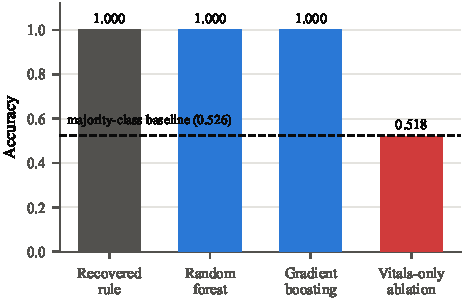
\includegraphics[width=\columnwidth]{figures/fig_audit.pdf}
\caption{Track A. Both ensembles reach the ceiling by recovering the label rule.
The ablation trained only on oxygen saturation, blood pressure, temperature and
respiratory rate falls \emph{below} the majority-class baseline: those channels
carry no information about the published label.}
\label{fig:audit}
\end{figure}

\subsection{Implication}

A classification score on this dataset measures recovery of
Equation~\ref{eq:rule}. It is not evidence of clinical predictive capability, and
reporting it as such would not survive a reviewer fitting a shallow tree. We
therefore do not use this dataset to train the deployed model.

%% ======================================================================
\section{Track B: Triage Under Sensor Noise}
\label{sec:trackb}

\subsection{The circularity problem}

Substituting NEWS2 for the dataset's label does not by itself solve anything.
NEWS2 is also a deterministic function of vital signs, so a model trained to
reproduce NEWS2 from clean vitals is learning a rule that is already known, and
any reported accuracy is a statement about function approximation.

\subsection{Design: latent truth versus observation}

We break the circularity by distinguishing what is true from what is measured:
\[
x^{*} \xrightarrow{\ \mathrm{NEWS2}\ } y^{*}, \qquad
x^{*} \xrightarrow{\ \text{sensor noise}\ } \hat{x},
\]
where $x^{*}$ is latent physiology, $y^{*}$ the ground-truth escalation band,
and $\hat{x}$ the corrupted telemetry. Ground truth is scored on $x^{*}$. Every
method---including the rule baseline---observes only $\hat{x}$. The rule
baseline computes NEWS2 on $\hat{x}$, which is precisely what a conventional
threshold monitor does. The learned model is trained on $(\hat{x}, y^{*})$ and
can therefore internalize the noise distribution and exploit cross-parameter
redundancy that a per-parameter rule cannot.

This yields a falsifiable comparison with a built-in negative control: at zero
noise $\hat{x} = x^{*}$, the rule is exact by construction, and the learned model
\emph{must not} beat it. Fig.~\ref{fig:design} shows the arrangement.

\begin{figure}[t]
\centering
% The latent/observed separation that makes Track B falsifiable.
%
% Deliberately carries no explanatory note: the caption states the negative
% control, and an in-diagram repetition collided with the method boxes.
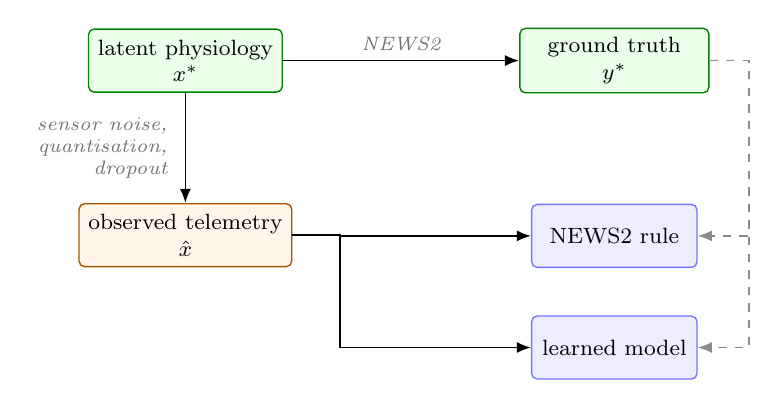
\begin{tikzpicture}[
    font=\footnotesize,
    box/.style   = {draw, rounded corners=2pt, minimum height=8mm,
                    minimum width=24mm, align=center, line width=0.5pt},
    truth/.style = {box, fill=green!8,  draw=green!50!black},
    obs/.style   = {box, fill=orange!8, draw=orange!65!black},
    meth/.style  = {box, fill=blue!7,   draw=blue!55, minimum width=21mm},
    arr/.style   = {-{Latex[length=1.8mm,width=1.4mm]}, line width=0.6pt},
    note/.style  = {font=\scriptsize\itshape, text=black!55, align=center},
  ]

  % Top row: the truth path, which no method ever observes.
  \node[truth] (latent) {latent physiology \\ $x^{*}$};
  \node[truth, right=30mm of latent] (y) {ground truth \\ $y^{*}$};
  \draw[arr] (latent) -- node[above, note] {NEWS2} (y);

  % Bottom row: the observation path, which every method does observe.
  \node[obs, below=14mm of latent] (obs) {observed telemetry \\ $\hat{x}$};
  \draw[arr] (latent) -- node[left, note, xshift=-1mm, align=right]
             {sensor noise, \\ quantisation, \\ dropout} (obs);

  \node[meth, below=14mm of y] (rule)  {NEWS2 rule};
  \node[meth, below=6mm of rule] (model) {learned model};

  \draw[arr] (obs.east) -- ++(6mm,0) |- (rule.west);
  \draw[arr] (obs.east) -- ++(6mm,0) |- (model.west);

  % Both methods are scored against the latent-signal ground truth. The dashed
  % edges carry this unlabelled: any text here overruns the column, and the
  % caption states it.
  \draw[arr, dashed, draw=black!45] (y.east) -- ++(5mm,0) |- (rule.east);
  \draw[arr, dashed, draw=black!45] (y.east) -- ++(5mm,0) |- (model.east);

\end{tikzpicture}

\caption{Separating latent physiology from sensor observation. Ground truth is
scored on the latent signal; every method, including the rule baseline, observes
only the corrupted telemetry; the dashed edges indicate that both are scored
against the same latent-signal truth. This is what makes ``learned model
versus threshold rule'' a real comparison rather than a restatement of the
labelling function.}
\label{fig:design}
\end{figure}

\subsection{Cohort and corruption model}

Latent severity is drawn from a three-component mixture (60\% stable, 25\% mild
derangement, 15\% acute deterioration) with four deterioration archetypes, so
channels move together as they do clinically rather than varying independently.
Corruption is applied per channel: Gaussian noise on all channels, motion
artifact on heart rate, perfusion dropout on oxygen saturation, display
quantization, and 3\% channel dropout imputed at inference. Train and test are
split by patient, never by row, since repeated readings from one simulated
patient are correlated.

\subsection{Metrics}

All estimators are implemented with scikit-learn~\cite{sklearn}.
Macro-F1 is the pre-registered selection criterion. It is insufficient alone: it
scores a missed high-risk observation identically to a spurious one. We
therefore also report high-risk recall, \emph{missed-HIGH} (the fraction of
high-risk observations reported as low risk), and a mean cost under an
asymmetric matrix penalizing under-triage far more heavily than over-triage.
Those weights are a stated assumption, not derived from outcome data.

\subsection{Results}

Table~\ref{tab:trackb} reports all five methods on the same corrupted
observations. Table~\ref{tab:noise} sweeps the noise scale, averaging three
independent cohort seeds per cell and reporting a 95\% confidence interval on
the model-minus-rule difference.

% generated by paper/make_tables.py -- do not edit
\begin{table*}[t]
\caption{Track B. Recovering the clean-signal NEWS2 band from sensor-corrupted
telemetry. All rows see the same corrupted observations. Missed-HIGH is the
fraction of HIGH observations reported as LOW.}
\label{tab:trackb}
\centering
\begin{tabular}{lrrrrr}
\toprule
Model & Accuracy & Macro-F1 & HIGH recall & Missed-HIGH & Mean cost \\
\midrule
news2\_rule\_on\_observed & 0.9005 & 0.8006 & 0.8847 & 0.0127 & 0.3165 \\
threshold\_alarms & 0.7352 & 0.6280 & 0.8520 & 0.0070 & 0.4461 \\
logistic\_regression & 0.8677 & 0.7866 & 0.8398 & 0.0023 & 0.2893 \\
random\_forest & 0.9005 & 0.8267 & 0.9013 & 0.0014 & 0.2074 \\
gradient\_boosting & 0.9260 & 0.8324 & 0.9199 & 0.0082 & 0.2651 \\
\bottomrule
\end{tabular}

\vspace{2pt}
\footnotesize Cohort: 120,000 readings from
30,000 simulated patients, split by patient.
Selection metric: \texttt{macro\_f1}. Macro-F1 selects \texttt{gradient\_boosting} while the asymmetric-cost criterion selects \texttt{random\_forest}; the F1-optimal model carries the higher rate of HIGH observations reported as LOW.
Cost weights are a stated assumption, not derived from outcome data.
\end{table*}

% generated by paper/make_tables.py -- do not edit
\begin{table}[t]
\caption{Macro-F1 against sensor-noise scale, mean over
3 independent cohort seeds. At $\sigma=0$ the observation
equals the latent signal, so the rule is exact and the learned model cannot
improve on it; the advantage appears only once observations are corrupted.}
\label{tab:noise}
\centering
\begin{tabular}{rrrrl}
\toprule
$\sigma$ & NEWS2 rule & gradient\_boosting & $\Delta$ & 95\% CI \\
\midrule
0.0 & 1.0000 & 0.9659 & -0.0341 & [-0.0381, -0.0300] \\
0.5 & 0.8669 & 0.8737 & +0.0067 & [+0.0030, +0.0105] \\
1.0 & 0.7976 & 0.8152 & +0.0177 & [+0.0158, +0.0195] \\
1.5 & 0.7362 & 0.7751 & +0.0390 & [+0.0277, +0.0502] \\
2.0 & 0.6819 & 0.7428 & +0.0609 & [+0.0553, +0.0665] \\
3.0 & 0.5855 & 0.6653 & +0.0798 & [+0.0644, +0.0951] \\
\bottomrule
\end{tabular}

\vspace{2pt}
\footnotesize $^{\dagger}$ interval includes zero; the difference is not
resolved at this number of seeds.
\end{table}


\begin{figure}[t]
\centering
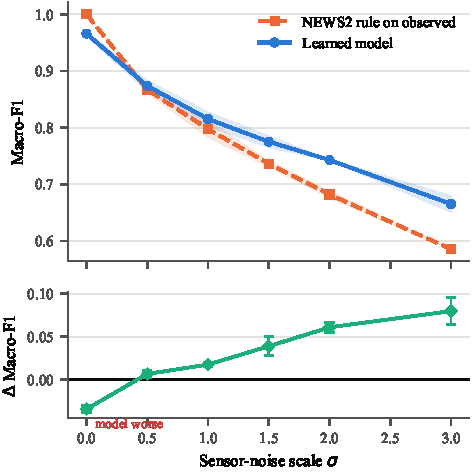
\includegraphics[width=\columnwidth]{figures/fig_noise_sweep.pdf}
\caption{Macro-F1 against sensor-noise scale (top) and the model-minus-rule
difference with 95\% confidence intervals over three cohort seeds (bottom).
Shaded bands are 95\% intervals. The difference changes sign: at $\sigma=0$ the
rule is exact and the learned model is significantly worse, and the advantage
appears only once observations are corrupted.}
\label{fig:noise}
\end{figure}

The negative control holds: at $\sigma = 0$ the rule is exact and the learned
model is significantly \emph{worse}. The advantage appears once observations are
corrupted and grows monotonically with noise, every interval excluding zero.
This is the paper's central empirical claim, and its credibility rests on the
fact that the design permits it to fail.

\subsection{Selection criteria disagree}

Macro-F1 and the cost criterion select different models. The F1-optimal model
attains higher aggregate scores while reporting high-risk observations as low
risk 5.9$\times$ more often than the cost-optimal alternative, for a macro-F1
difference of less than $0.006$. We report the disagreement and retain the
pre-registered criterion; changing it after observing results would be precisely
the post-hoc selection that makes a reported number untrustworthy.

\subsection{Calibration}

The system displays a confidence value, so whether that value means anything is
part of the result rather than an implementation detail.
Table~\ref{tab:calibration} gives the reliability table.

% generated by paper/make_tables.py -- do not edit
\begin{table}[t]
\caption{Calibration of the selected triage model. A positive gap means stated
confidence exceeds observed accuracy in that bin.}
\label{tab:calibration}
\centering
\begin{tabular}{lrrrr}
\toprule
Confidence bin & $n$ & Mean conf. & Accuracy & Gap \\
\midrule
{}[0.3, 0.4] & 26 & 0.387 & 0.500 & -0.113 \\
{}[0.4, 0.5] & 414 & 0.471 & 0.454 & +0.016 \\
{}[0.5, 0.6] & 1,054 & 0.550 & 0.548 & +0.001 \\
{}[0.6, 0.7] & 1,063 & 0.651 & 0.611 & +0.039 \\
{}[0.7, 0.8] & 1,009 & 0.751 & 0.733 & +0.018 \\
{}[0.8, 0.9] & 1,283 & 0.853 & 0.843 & +0.010 \\
{}[0.9, 1.0] & 19,151 & 0.988 & 0.991 & -0.002 \\
\bottomrule
\end{tabular}

\vspace{2pt}
\footnotesize ECE 0.0053, MCE 0.1131,
Brier 0.1022, overall over-confidence
+0.0014.
\end{table}


\begin{figure}[t]
\centering
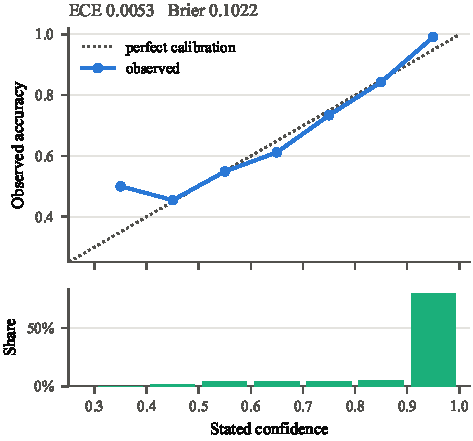
\includegraphics[width=\columnwidth]{figures/fig_calibration.pdf}
\caption{Reliability diagram for the selected triage model, with bin support
below. Points on the diagonal indicate that a stated confidence matches observed
accuracy. Support is shown because a large gap in a sparsely populated bin is a
weaker finding than the same gap in a well populated one.}
\label{fig:calibration}
\end{figure}

\subsection{Sensor-only deployment}

Two NEWS2 parameters---supplemental oxygen and consciousness---are recorded by
staff, not sensed by a wearable. A deployment fed only by wearables cannot supply
them, and the interface defaults them to the benign case.
Table~\ref{tab:wearable} quantifies the resulting silent train/serve mismatch and
shows that retraining for the inputs actually present recovers most of the
safety margin while barely changing macro-F1---another instance of the aggregate
metric concealing the clinically relevant difference.

% generated by paper/make_tables.py -- do not edit
\begin{table}[t]
\caption{Wearable-only deployment ablation. Supplemental oxygen and AVPU are
NEWS2 parameters that a wearable cannot supply.}
\label{tab:wearable}
\centering
\begin{tabular}{lrrr}
\toprule
Scenario & Macro-F1 & HIGH recall & Missed-HIGH \\
\midrule
Full observation (reported setting) & 0.8214 & 0.8891 & 0.0051 \\
Trained full, served wearable-only & 0.7783 & 0.7803 & 0.0167 \\
Trained and served wearable-only & 0.7744 & 0.8448 & 0.0109 \\
\bottomrule
\end{tabular}

\vspace{2pt}
\footnotesize Serving the fully-trained model on a wearable-only feed costs
+0.0431 macro-F1 and raises missed-HIGH by
+0.0116.
\end{table}


\begin{figure}[t]
\centering
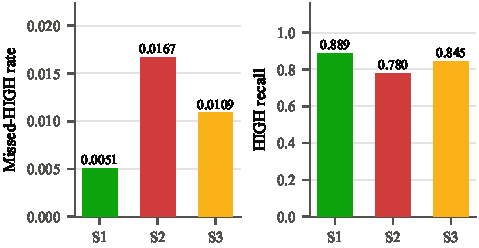
\includegraphics[width=\columnwidth]{figures/fig_wearable.pdf}
\caption{Sensor-only deployment. Serving the fully-trained model against a feed
lacking supplemental-oxygen and consciousness observations (S2) raises the rate
of high-risk observations reported as low risk more than three-fold. Retraining
for the inputs actually present (S3) recovers most of the safety margin while
barely changing macro-F1.}
\label{fig:wearable}
\end{figure}

%% ======================================================================
\section{System Architecture}
\label{sec:arch}

\subsection{Overview}

Four components: a Python triage service exposing a stateless inference API; a
Java backend owning authentication, validation, persistence, orchestration and
the summarization cascade; PostgreSQL for durable telemetry and assessments; and
a browser dashboard. Fig.~\ref{fig:arch} shows the arrangement and, more
importantly, the boundary between what must be fast and what is permitted to be
slow.

\begin{figure*}[t]
\centering
% System architecture and data flow.
% Hand-authored TikZ (structure, not data). Data figures are generated by
% paper/make_figures.py from the experiment artifacts.
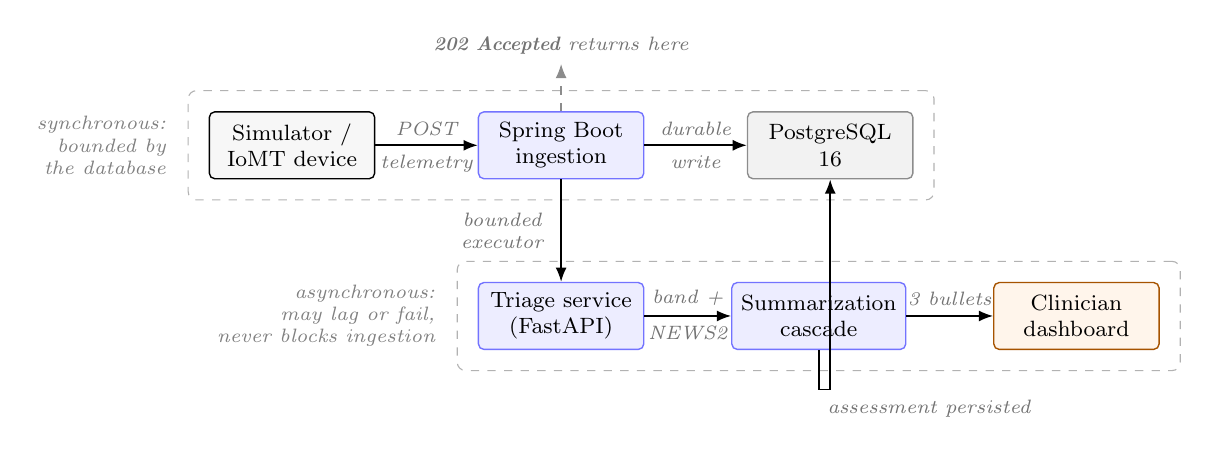
\begin{tikzpicture}[
    font=\footnotesize,
    box/.style   = {draw, rounded corners=2pt, minimum height=8.5mm,
                    minimum width=21mm, align=center, line width=0.5pt},
    svc/.style   = {box, fill=blue!7,  draw=blue!55},
    store/.style = {box, fill=black!5, draw=black!45},
    ui/.style    = {box, fill=orange!8, draw=orange!65!black},
    arr/.style   = {-{Latex[length=1.8mm,width=1.4mm]}, line width=0.6pt},
    note/.style  = {font=\scriptsize\itshape, text=black!55, align=center},
    zone/.style  = {font=\scriptsize\itshape, text=black!50},
  ]

  % --- row 1: the synchronous ingestion path -----------------------------
  \node[box, fill=black!3] (dev) {Simulator /\\IoMT device};
  \node[svc, right=13mm of dev] (api) {Spring Boot\\ingestion};
  \node[store, right=13mm of api] (db) {PostgreSQL\\16};

  \draw[arr] (dev) -- node[above, note] {POST}
                      node[below, note] {telemetry} (api);
  \draw[arr] (api) -- node[above, note] {durable}
                      node[below, note] {write} (db);

  % The claim: ingestion answers before any analysis has happened.
  \node[note, above=6mm of api] (accepted) {\textbf{202 Accepted} returns here};
  \draw[arr, dashed, draw=black!45] (api.north) -- (accepted.south);

  % --- row 2: the asynchronous analysis path -----------------------------
  \node[svc, below=13mm of api] (ml) {Triage service\\(FastAPI)};
  \node[svc, right=11mm of ml]  (casc) {Summarization\\cascade};
  \node[ui,  right=11mm of casc] (dash) {Clinician\\dashboard};

  \draw[arr] (api.south) -- node[left, note, xshift=-1mm]
             {bounded\\executor} (ml.north);
  \draw[arr] (ml) -- node[above, note] {band +} node[below, note] {NEWS2} (casc);
  \draw[arr] (casc) -- node[above, note] {3 bullets} (dash);
  \draw[arr] (casc.south) -- ++(0,-5mm)
             node[below, note, xshift=14mm] {assessment persisted} -| (db.south);

  % --- the separation being asserted -------------------------------------
  % Zone labels sit outside the dashed boxes: placed on the frame they collide
  % with the nodes inside.
  \begin{scope}[on background layer]
    \node[draw=black!30, dashed, rounded corners=3pt, inner sep=2.6mm,
          fit=(dev)(api)(db)] (sync) {};
    \node[draw=black!30, dashed, rounded corners=3pt, inner sep=2.6mm,
          fit=(ml)(casc)(dash)] (async) {};
  \end{scope}

  \node[zone, left=1.5mm of sync.west, anchor=east, align=right]
       {synchronous:\\bounded by\\the database};
  \node[zone, left=1.5mm of async.west, anchor=east, align=right]
       {asynchronous:\\may lag or fail,\\never blocks ingestion};

\end{tikzpicture}

\caption{Architecture and the synchronous/asynchronous boundary. Ingestion
performs one durable write and returns \texttt{202 Accepted}; triage and
summarization proceed on a bounded executor behind it. Ingestion throughput is
therefore bounded by the database, never by whichever language model is
currently answering.}
\label{fig:arch}
\end{figure*}

\subsection{The decoupling rule}

Telemetry ingestion performs validation and one durable write, then returns
\texttt{202 Accepted}. Analysis is handed to a bounded executor with a
caller-runs rejection policy, so sustained overload applies backpressure to
ingestion instead of growing an unbounded queue of pending model calls.
Ingestion throughput is bounded by the database, never by whichever language
model is currently answering.

\subsection{Summarization cascade}

Generation is attempted best-first: a local model, then a cloud model, then a
deterministic template generator with no external dependency. Each tier may fail
or time out; the terminal tier cannot, which is what makes the cascade total.
The tier that answered and its latency are persisted per assessment, so
resilience is measured from stored data rather than inferred from logs.
Fig.~\ref{fig:cascade} shows the flow, including the faithfulness gate described
below.

\begin{figure}[t]
\centering
% Summarization cascade. The terminal tier is what makes the cascade total.
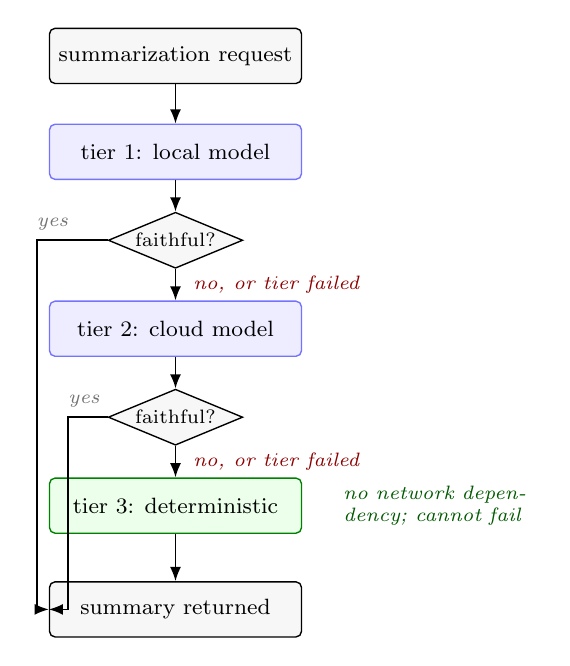
\begin{tikzpicture}[
    font=\footnotesize,
    node distance=5mm,
    tier/.style  = {draw, rounded corners=2pt, minimum height=7mm,
                    minimum width=32mm, align=center, line width=0.5pt},
    llm/.style   = {tier, fill=blue!7,  draw=blue!55},
    det/.style   = {tier, fill=green!8, draw=green!50!black},
    gate/.style  = {draw, diamond, aspect=2.4, inner sep=0.4mm, fill=black!3,
                    align=center, font=\scriptsize, line width=0.5pt},
    arr/.style   = {-{Latex[length=1.8mm,width=1.4mm]}, line width=0.6pt},
    note/.style  = {font=\scriptsize\itshape, text=black!55, align=left},
    fail/.style  = {note, text=red!55!black},
  ]

  \node[tier, fill=black!3] (req) {summarization request};
  \node[llm, below=of req]  (ollama) {tier 1: local model};
  \node[gate, below=4mm of ollama] (g1) {faithful?};
  \node[llm, below=4mm of g1] (gemini) {tier 2: cloud model};
  \node[gate, below=4mm of gemini] (g2) {faithful?};
  \node[det, below=4mm of g2] (rule) {tier 3: deterministic};
  \node[tier, fill=black!3, below=6mm of rule] (out) {summary returned};

  \draw[arr] (req)    -- (ollama);
  \draw[arr] (ollama) -- (g1);
  \draw[arr] (g1)     -- node[right, fail, xshift=1mm] {no, or tier failed} (gemini);
  \draw[arr] (gemini) -- (g2);
  \draw[arr] (g2)     -- node[right, fail, xshift=1mm] {no, or tier failed} (rule);
  \draw[arr] (rule)   -- (out);

  % Success paths bypass the remaining tiers.
  \draw[arr] (g1.west) -- ++(-9mm,0) node[above, note, xshift=2mm] {yes}
             |- (out.west);
  \draw[arr] (g2.west) -- ++(-5mm,0) node[above, note, xshift=2mm] {yes}
             |- (out.west);

  \node[note, right=4mm of rule, text width=24mm, text=green!35!black]
       {no network dependency; cannot fail};

\end{tikzpicture}

\caption{Summarization cascade. A tier that fails, times out, or returns output
failing the faithfulness check is skipped. The deterministic tier has no
external dependency and therefore always produces a summary, which is the
property the availability claim rests on.}
\label{fig:cascade}
\end{figure}

\subsection{Faithfulness enforcement}

Prompt instructions are not enforcement. Generated text is mechanically checked
before acceptance: every number it cites must correspond to a supplied value
within a tolerance that admits rounding but not fabrication, and no named
condition may appear. Output failing either check is treated as a tier failure
and the cascade falls through. Deterministic output is checked by the same guard
and is verified in test to always pass.

This is necessary, not sufficient. It catches invented values; it cannot detect a
fluent, numerically correct, clinically wrong interpretation.

%% ======================================================================
\section{System Evaluation}

\subsection{Triage latency}

Triage is the only model-dependent step in the synchronous-facing path, so its
cost bounds how much of the ingestion budget analysis can consume.
Table~\ref{tab:latency} reports the in-process model call over 1000
single-observation predictions. The distribution is tight and the tail is
short, which is what permits analysis to be scheduled per reading rather than
batched.

% generated by paper/make_tables.py -- do not edit
\begin{table}[t]
\caption{Triage inference latency, 1000 single-observation predictions.
In-process model call only: excludes HTTP, serialisation and network transit.}
\label{tab:latency}
\centering
\begin{tabular}{lr}
\toprule
Statistic & Milliseconds \\
\midrule
Mean & 2.758 \\
p50 & 2.684 \\
p95 & 3.719 \\
p99 & 4.297 \\
Maximum & 4.687 \\
\bottomrule
\end{tabular}

\vspace{2pt}
\footnotesize Measured on one developer workstation. Not a service-level
objective.
\end{table}


\subsection{Decoupling under a stalled dependency}

With the triage service artificially stalled for 3\,s, ingestion returns in under
1\,s. A synchronous implementation cannot pass this test, which is why it is the
load-bearing test of the architectural claim.

\subsection{Throughput}

Offered load was generated open-loop, so a server falling behind manifests as
rising latency rather than a silently reduced offered rate. At 10, 50 and 100
requests per second the system tracks the offered rate with p95 ingestion
latency between 27 and 31\,ms. At an offered 250 it saturates, achieving
approximately 159 requests per second with p95 latency rising to several
seconds. The asynchronous analysis backlog drained completely at every rate.
Fig.~\ref{fig:throughput} shows both panels; achieved rate and latency are
plotted separately rather than on twin axes, since they share no scale.

\begin{figure}[t]
\centering
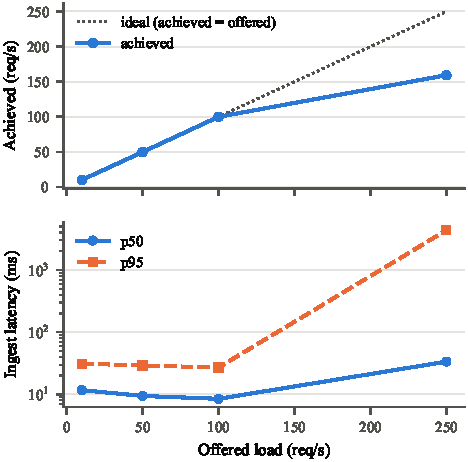
\includegraphics[width=\columnwidth]{figures/fig_throughput.pdf}
\caption{Ingestion under open-loop offered load. Achieved rate tracks offered
load to 100 requests per second and then departs from it; p95 latency rises by
two orders of magnitude at the saturation point. Latency uses a logarithmic
axis.}
\label{fig:throughput}
\end{figure}

\subsection{Resilience}

Three conditions were exercised by stopping and restarting containers. With all
services running, every reading produced an assessment. With the triage service
stopped, ingestion and summarization both remained at 100\%, assessments being
recorded with the model marked unavailable and summaries produced by the
deterministic tier. On restart the system resumed using the model without a
backend restart.

\subsection{Notification event counts}

% generated by paper/make_tables.py -- do not edit
\begin{table}[t]
\caption{Notification event counts over 4,800
simulated readings. A emits one event per breaching parameter per reading; B one
per reading whose band is not LOW; C one per upward band transition per patient.
This is event arithmetic only.}
\label{tab:events}
\centering
\begin{tabular}{lrr}
\toprule
Policy & Events & Per 100 \\
\midrule
A. Per-parameter thresholds & 4,306 & 89.71 \\
B. Aggregate band & 1,262 & 26.29 \\
C. Band transition & 419 & 8.73 \\
\bottomrule
\end{tabular}

\vspace{2pt}
\footnotesize \textbf{These counts are not a measurement of alert
fatigue, clinician workload, or patient benefit.} Policy C emits fewer
notifications by construction; whether that is clinically safe is untested here.
\end{table}


We stress that this is arithmetic over a simulated stream. It is not a
measurement of alert fatigue, clinician workload, or patient benefit, and it must
not be read as one. A policy emitting fewer notifications is not thereby safer;
fewer notifications can mean missed deterioration.

%% ======================================================================
\section{Live Language Model Evaluation}
\label{sec:llm}

This section reports the behaviour of the live summarization tiers. Two
generative tiers were enabled: a local tier, \texttt{llama3.1:8b} served by
Ollama on the evaluation host, and a cloud tier, \texttt{gemini-3.1-flash-lite}.
The deterministic tier was retained as the terminal fallback. Thirty synthetic
assessments spanning the severity range were submitted through the ordinary
assessment path, so each observation traversed the same cascade a caller would
exercise. Table~\ref{tab:llm} reports the result.

% generated by paper/make_tables.py -- do not edit
\begin{table}[t]
\caption{Live summarization cascade over 30 cases spanning the
severity range. Faithfulness is computed over a tier's own attempts: the share
that cited only supplied numbers and named no condition. A rejected summary is
never returned, so it is the attempt count, not the answered count, that makes
this rate informative.}
\label{tab:llm}
\centering
\begin{tabular}{lrrrrrr}
\toprule
Tier & Att. & Rej. & Faith. & Ans. & Share & p50 (ms) \\
\midrule
ollama & 30 & 10 & 0.667 & 20 & 66.7\% & 10130.8 \\
gemini & 10 & 0 & 1.000 & 10 & 33.3\% & 18881.6 \\
\bottomrule
\end{tabular}

\vspace{2pt}
\footnotesize Tiers enabled: ollama, gemini. Att.\ is attempts, Rej.\ summaries
the faithfulness guard rejected, Ans.\ those returned to the caller. A
rejected summary causes the cascade to fall through to the next tier, so
rejections at one tier appear as attempts at the next. Faithfulness checking is
necessary, not sufficient: it cannot detect a fluent, numerically correct,
clinically wrong reading of the data.
\end{table}


The local tier attempted all thirty assessments and answered twenty. The
faithfulness guard rejected the remaining ten, every one of which fell through
to the cloud tier, which answered all ten and was rejected on none. The
deterministic tier was never reached. No tier timed out or returned an error
during the run, so every fallthrough observed was a faithfulness rejection
rather than an availability failure.

The headline figure is that the local tier's output was rejected on one third
of its attempts. The rejections were not malformed text: in each case the model
produced a fluent summary that cited a numeric value absent from the
observation it was given, including plausible vital signs such as a temperature
of $37.5^{\circ}$C, a respiratory rate of 16 and an oxygen saturation of 95\%.
These are the values a reader would be least likely to question. The guard
rejects on provenance rather than plausibility, which is why it catches them.

This measurement requires one methodological note. The rate reported here is
computed over each tier's \emph{attempts}, recorded by instrumenting the
cascade directly. A rate computed over returned summaries cannot fall below
unity, because a summary that fails the guard is never returned; such a figure
would be a restatement of the guard's definition rather than a measurement of
model behaviour. The distinction matters: over this run the attempt-based rate
for the local tier is $0.667$, while the returned-summary rate for the same
tier is $1.000$.

Three limits apply to these figures. They describe a single run of thirty
synthetic cases on one host, and are not a stability estimate; a repeat run
under the same configuration produced eight rejections rather than ten. The
fallthrough rate is a property of this model pair at this prompt, and a
different local model would move it. And as Section~\ref{sec:limits} records,
the guard is a provenance check over numbers and condition names: it cannot
detect a summary that is fluent, numerically correct and clinically wrong.

What the run does establish is that the guard is load-bearing rather than
decorative. On this model pair it fired on a third of local-tier attempts, and
on every occasion the cascade recovered without returning fabricated content to
the caller.


%% ======================================================================
\section{Discussion}

\subsection{On auditing before modeling}

The Track A finding was not subtle and required no sophisticated tooling---a
depth-3 tree exposes it in seconds. It survives in the literature because the
standard workflow never asks the question. We suggest that any classification
result on a public physiological dataset should be accompanied by evidence that
the label is not a deterministic function of the features, and that this is
cheap enough to be routine.

\subsection{On negative controls}

The $\sigma = 0$ result, where the learned model is significantly worse than the
rule, is the most informative number in Table~\ref{tab:noise}. A design in which
the model wins everywhere would be indistinguishable from a design that leaks.

\subsection{On aggregate metrics in clinical triage}

Macro-F1 selected the worse model twice, under different circumstances: once
between estimator families, once between input configurations. In both cases the
cost-relevant difference was invisible in the aggregate score. This is an
argument for reporting directional error rates alongside aggregate metrics
whenever error costs are asymmetric.

%% ======================================================================
\section{Limitations}

\begin{enumerate}
  \item The Track B cohort is simulated. Results are software evaluation, not
        clinical validation, and the corruption model is a stated assumption.
  \item The live model evaluation in Section~\ref{sec:llm} is a single run
        of thirty synthetic cases against one model pair on one host. It
        establishes that the faithfulness guard fires against real
        generative output, but the rejection rate is not a stable estimate
        and does not transfer to other models or prompts.
  \item Faithfulness checking cannot detect fluent, numerically correct,
        clinically incorrect interpretation.
  \item The asymmetric cost weights encode intuition, not outcome data.
  \item NEWS2 is validated for acutely ill adults in hospital; applying it to
        simulated continuous wearable telemetry is outside its validation scope.
  \item Security is prototype grade: a single demo credential, no refresh or
        revocation, no external identity provider, no TLS in the bundled stack.
  \item Throughput figures characterize one workstation and are not service
        level objectives.
\end{enumerate}

%% ======================================================================
\section{Ethics and Safety}

The system is a research prototype and not a medical device. It produces
software triage categories, not diagnoses, and every response carries that
statement. No real patient data was used at any stage; all cohorts are simulated
and the audited public dataset contains no identifiable information. Enabling the
cloud summarization tier transmits telemetry to a third party, which is
acceptable for synthetic data and would require a data processing agreement
otherwise. Deployment on real data would require the hardening enumerated under
Limitations, and a determination of regulatory status under applicable Clinical
Decision Support guidance.

%% ======================================================================
\section{Reproducibility}

All results are regenerated from a clean checkout by \texttt{run\_all.sh} or
\texttt{run\_all.ps1}. Each experiment writes a JSON artifact recording its
seeds, configuration and environment; every table in this paper is generated
from those artifacts by \texttt{paper/make\_tables.py}, and no number is entered
by hand. The audited dataset is not redistributed; a resolver script locates it
and records its SHA-256 so a result can be tied to a specific file. Track B
requires no external data.

%% ======================================================================
\section{Conclusion}

VitalSync demonstrates that continuous telemetry ingestion and low-latency risk
triage can be isolated from generative summarization, remaining fully available
when every language model tier is unreachable. Along the way we found that the
public dataset the work was premised on carries a label that is a deterministic
rule over two variables, and we report that as a caution about label provenance.
Separating latent physiology from sensor observation gives a falsifiable
comparison in which a learned model outperforms a threshold rule only under
observation noise---and demonstrably fails to when there is none. Finally, we
show that aggregate classification metrics can select triage models that are
materially worse under asymmetric clinical cost. Evaluating the generative tiers
themselves remains open, and is marked as such.

\section*{Acknowledgment}

The authors used an AI coding assistant for implementation and analysis
scaffolding. All reported measurements were produced by executing the referenced
code, and the artifacts are included.

\begin{thebibliography}{00}

\bibitem{rcp2019} Royal College of Physicians, ``National Early Warning Score
(NEWS) 2: Standardising the assessment of acute-illness severity in the NHS,''
RCP, London, 2017.

\bibitem{fhir} HL7 International, ``FHIR R4: Observation Resource,''
\url{https://hl7.org/fhir/R4/observation.html}.

\bibitem{nist} National Institute of Standards and Technology, ``Artificial
Intelligence Risk Management Framework: Generative Artificial Intelligence
Profile,'' NIST AI 600-1, 2024.

\bibitem{fda} U.S. Food and Drug Administration, ``Clinical Decision Support
Software: Guidance for Industry and Food and Drug Administration Staff.''

\bibitem{rpm} ``Patient outcomes associated with continuous remote patient
monitoring: a scoping review,'' 2025.

\bibitem{llmsum} ``Scientific evidence for clinical text summarization using
large language models: scoping review,'' \emph{J. Med. Internet Res.}, 2025.

\bibitem{sklearn} F. Pedregosa et al., ``Scikit-learn: Machine learning in
Python,'' \emph{J. Mach. Learn. Res.}, vol. 12, pp. 2825--2830, 2011.

\bibitem{dataset} N. Ayub, ``Human Vital Sign Dataset,'' Kaggle, 2024.
\url{https://www.kaggle.com/datasets/nasirayub2/human-vital-sign-dataset}.
Audited in Section~\ref{sec:tracka}; its risk label is a deterministic rule.

\bibitem{arrhythmia_2025} ``A Resource-Efficient Cardiac Arrhythmia Detection Using Nonlinear Dynamics in Optimized Delay State Networks,'' \emph{IEEE Transactions on Biomedical Engineering}, 2025.

\bibitem{iot_offloading_2025} ``Generative AI-Aided Multimodal Parallel Offloading for Edge Services in IoT Networks,'' \emph{IEEE Transactions on Internet of Things}, 2025.

\bibitem{fed_llm_2026} ``Dynamic Resource Allocation for Federated Large Language Models in the Internet of Medical Things: A DRL Approach,'' \emph{IEEE Transactions on Mobile Computing}, 2026.

\bibitem{mealmeter_2025} ``MealMeter: AI-Driven Multimodal Health Tracking Using Wearable Sensors and Deep Feature Fusion,'' \emph{IEEE Transactions on Biomedical Engineering}, 2025.

\bibitem{privacy_llm_smart_2026} ``Privacy-Preserving Adaptive Differential Privacy for Large Language Models in Smart Healthcare,'' \emph{IEEE Transactions on Information Forensics and Security}, 2026.

\bibitem{alert_fatigue_2024} ``Alert Fatigue in Electronic Health Records: Cognitive Load and Clinical Decision-Making,'' \emph{Journal of Medical Internet Research}, 2024.

\bibitem{fog_iot_2024} ``Fog Computing for Real-Time Healthcare IoT: Latency Optimization and Data Privacy,'' \emph{IEEE Journal on Biomedical and Health Informatics}, 2024.

\bibitem{nlp_clinical_2025} ``Natural Language Processing for Clinical Documentation: Automated Summarization of Patient Telemetry,'' \emph{Journal of Biomedical Informatics}, 2025.

\bibitem{microservices_2024} ``Microservices Architecture in Healthcare Systems: Scalability, Resilience, and Decoupling Benefits,'' \emph{ACM Transactions on Computing for Healthcare}, 2024.

\bibitem{dp_llm_healthcare_2025} ``Differential Privacy in Large Language Models for Healthcare: Balancing Utility and Protection,'' \emph{Nature Machine Intelligence}, 2025.

\bibitem{wearable_review_2024} ``Wearable Sensor Data Integration in Clinical Decision Support: A Systematic Review,'' \emph{Computers in Biology and Medicine}, 2024.

\end{thebibliography}

\end{document}
